\documentclass{../../../fal_assignment}
\graphicspath{ {../../../} }

\usepackage{enumitem}
\setlist{nosep} % Make enumerate / itemize lists more closely spaced
\usepackage[T1]{fontenc} % http://tex.stackexchange.com/a/17858
\usepackage{url}
\usepackage{todonotes}

\title{COMP140 Worksheet C: Arduino based Pong controller}
\author{Alcwyn Parker}
\module{COMP140}

\begin{document}

\maketitle



\section*{Introduction}

In this worksheet, you will use an Arduino to create a game controller for the retro arcade classic, Pong. The source for the game exists already. You are tasked with modifying the code to include bidirectional communication with the Arduino. The suggested design of the final controller is: two potentiometers to control the paddles and some combination of LEDs that flash when someone scores. Feel free to add some creative flair to the suggested design or modify it completely. The only requirement is that there must be two-way communication between the Arduino and the game. The wiring diagram below shows a potential controller setup for this worksheet. You are encouraged to create the controller one step at a time following the steps below. \textbf{DO NOT} wire everything up in one go and then expect it to work first time. 

\begin{figure}[!h]
	\begin{center}
		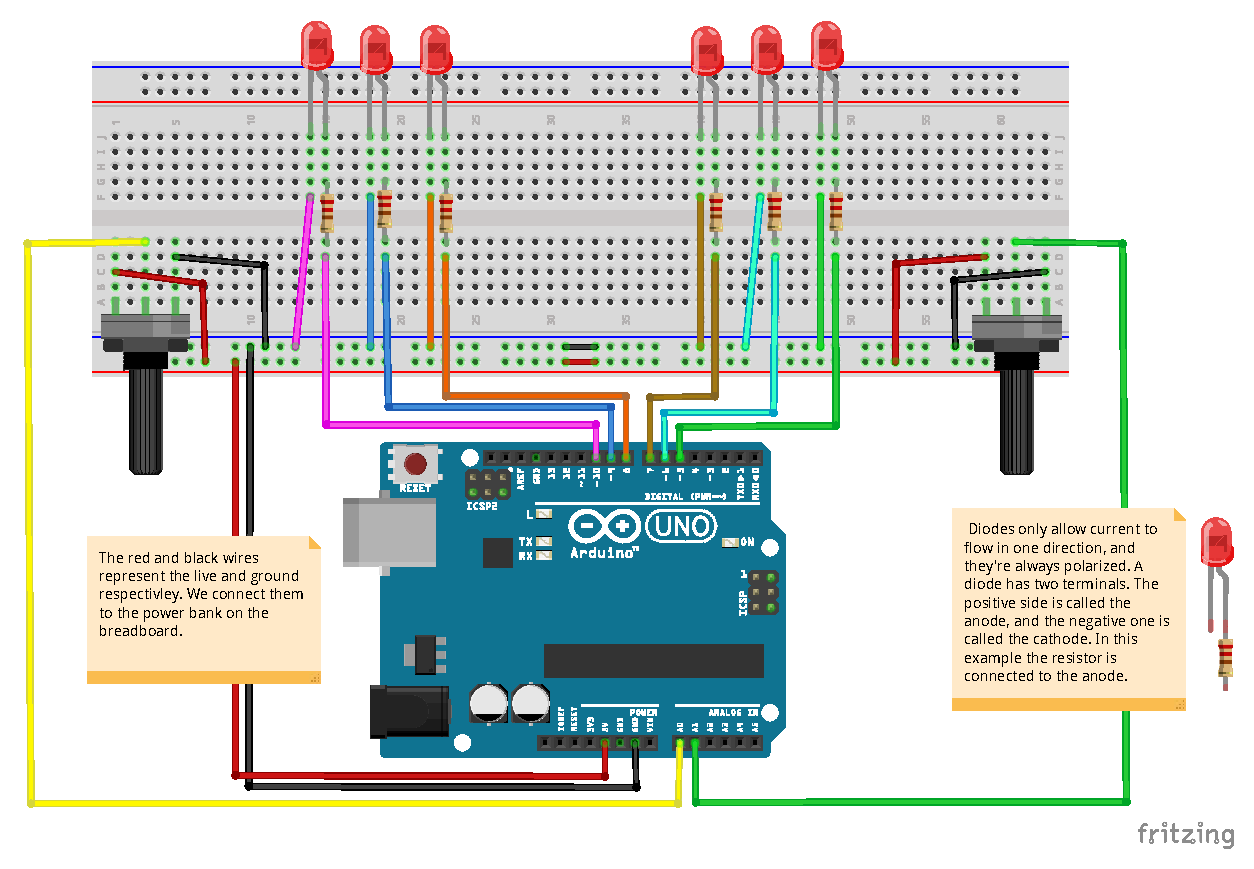
\includegraphics[width=0.9\textwidth]{assets/arduino-pong.pdf}
	\end{center}
	\caption{Pong Controller Wiring Diagram}
	\label{fig:wiring}
\end{figure}

\section{A Single Potentiometer} \label{arduino-first}
To begin, connect one potentiometer to the breadboard. Hook the potentiometer up to the Arduino. Then write an Arduino sketch to send the potentiometer values over the serial connection. Tested this works using the serial monitor built into the Arduino IDE. Then, adapt the Pong source to update player one's paddle using the values from the potentiometer. 

\section{Two Potentiometers} \label{arduino-second}
Mirror the potentiometer wiring for the second player and alter the code to send the values of both potentiometers delimited by a hyphen. Update the Pong code so that it splits the values received over serial and uses the first value to control the left paddle and the second value to control the right paddle. 

\section{Visual Feedback - Part 1} \label{arduino-third}
Now that the player control is finished, we need to start thinking about visual feedback. Create the circuit for one of the LEDs in the diagram above. It doesn't matter which one but for simplicity lets say it is the LED attached to digital pin 8. Update the Arduino sketch so that if serial communication is received and the byte read represents a capital 'L' then the LED attached to pin number 8 flashes. Wire up a second LED but this time connect it to pin 7. Update the Arduino sketch so that if serial communication is received and the byte read represents a capital 'R' then the LED attached to pin number 7 flashes. Test the LEDs using the serial monitor in the Arduino IDE. 

\section{Visual Feedback - Part 2} \label{arduino-fourth}
Once you have tested that the LEDs work as is expected, modify the Pong code so that LEDs can be triggered to flash. When player one scores a point send an 'L' to the Arduino and when player to scores a point send an 'R'.

\marginpicture{flavour_pic}{
    Example setup
}


\section*{Submission instructions}

Begin by \textbf{forking} the GitHub repository at the following URL:

\url{https://github.com/Falmouth-Games-Academy/comp140-worksheetc}

You should complete a pull request before the hand-in on Friday by 5pm on Week 5. Feedback will be given in the pull request and in class.

\section*{Marking criteria}

Remember that \textbf{it is better to submit incomplete work than to submit nothing at all}. 

To demonstrate \textbf{basic competency}, complete the following:
\begin{itemize}
	\item Connect one potentiometer to the breadboard. Hook the potentiometer up to the Arduino
	\item Send the value read from the potentiometer to the Serial.
	\item Modify the Pong code to read the value from serial and update player one's paddle accordingly.
\end{itemize} 

To demonstrate \textbf{basic proficiency}, complete the following:
\begin{itemize}
	\item Achieve \textbf{basic competency}.
	\item Mirror the potentiometer setup for player two.
	\item Modify the Pong code to read the value from serial and update player one and player two's paddle accordingly.
\end{itemize}

To demonstrate \textbf{novice competency}, complete the following:
\begin{itemize}
	\item Achieve \textbf{basic proficiency}.
	\item Create the circuits for two LEDs.
	\item Make the LEDs flash using the serial monitor built into the Arduino IDE.
\end{itemize}

To demonstrate \textbf{novice proficiency}, complete the following:
\begin{itemize}
	\item Achieve \textbf{novice competency}
	\item Modify the Pong code so that it can trigger the LEDs to flash.
	\item add some creative flair to the visual feedback
\end{itemize}

To demonstrate \textbf{professional competency}, complete the following:
\begin{itemize}
	\item Achieve \textbf{novice proficiency}
	\item Enhance the visual feedback so that it can communicate a best of three scenario.
\end{itemize}


\end{document}
